\section{Méthodes de résolution des facteurs de vue}

Une grande diversité des méthodes de résolution des facteurs de vue existe. L'objectif de cette étude n'est pas de comparer les méthodes, mais d'utiliser les plus efficaces dans un contexte de géométries complexes. Ainsi le travail de synthèse de Manoj Kumar Gupta et al. \cite{methods_fv} souligne l'incompatibilité des méthodes de \itt{Hottel's cross string} et \itt{Unit Sphere and Hemicube Method} développée dans \cite{Howell185} dans un contexte de réacteurs français ou européens. La première méthode est utile en cas de milieu semi infini \cite{Hajji2015} ou par exemple pour des géométries caractéristiques des réacteurs à lit de boulets (\itt{Pebled Bed Reactor}) \cite{pbr9}. La deuxième méthode de sphère unité a la belle charactéristique de pouvoir être évaluée expérimentalement mais n'atteint pas des seuils de précision nécessaires à notre étude. 

La diversité des méthodes restantes, développées dans \cite{Howell} ne sera pas abordées en profondeur. La méthode retenue est la méthode de Monte Carlo Ray Tracing. Deux autres méthodes sont présentées afin de comprendre comment sont établis des facteurs de vue pour des géométries simples.

La première sous partie développe un exemple de résolution directe de l'intégrale et montre la limitation de cette méthode bien qu'elle soit la plus précise. La seconde sous partie donne les grandes lignes d'une résolution astucieuse des facteurs de vue dans des géométries arrageantes. Enfin la dernière sous partie insistera sur la méthode Monte-Carlo comme méthode de référence pour une géométrie complexe. 

\subsection{Méthode d'intégration directe : résolution de l'intégrale}
Afin d'évaluer la faisabilité d'une résolution intégrale directe des facteurs de vue, le cas du facteur de vue entre deux faces opposées d'un cube unité est développée en Annexe \ref{anx:int}. À partir de la définition intégrale du facteur de vue, le problème conduit initialement à une intégrale quadruple portant sur l'ensemble des paires de points appartenant aux deux surfaces.

L'exploitation de la géométrie du problème permet toutefois de simplifier significativement cette expression. En introduisant les coordonnées relatives entre les deux faces et en utilisant une propriété de convolution, l'intégrale quadruple est ramenée à une intégrale double sur les distances relatives. Cette transformation met en évidence un facteur de pondération géométrique représentant la densité des paires de points associées à une même séparation.

L'intégrale obtenue est ensuite traitée analytiquement par introduction d'une fonction auxiliaire dépendant d'un paramètre, puis par décomposition du terme de pondération en contributions élémentaires. Cette démarche conduit à une expression analytique fermée du facteur de vue entre deux faces opposées du cube :

\begin{equation}
F_{16}=\frac{2}{\pi} \left[ \ln(\frac{2}{\sqrt{3}}) +2\sqrt{2}arctan(\frac{1}{\sqrt{2}})-\frac{\pi}{2} \right]
\end{equation}

La valeur numérique obtenue est :
\begin{equation}
F_{12}\simeq 0.1998.
\end{equation}

Ce résultat montre qu'une résolution intégrale directe est réalisable pour des géométries simples et fortement symétriques. Néanmoins, la complexité des manipulations analytiques nécessaires, même dans le cas élémentaire du cube, illustre les difficultés d'une telle approche pour des géométries plus générales. Cette observation justifie le recours à des méthodes numériques dédiées au calcul des facteurs de vue dans les configurations complexes.

\subsection{Méthode algébrique : utilisation des propriétés géométriques}
Une version aussi élégante que limitée permet de trouver les facteurs de vue en utilisant la réciprocité, la complémentarité et la symétrie de ces derniers.
\subsubsection*{Utilisation de la réciprocité}
Les facteurs de vue pour deux sphères concentriques sont se retrouvent de manière assez directes. La face intérieure éclaire complètement la face extérieur. Par réciprocité, on obtient $ F_{out->in} = \frac{S_{in}}{S_{out}} \times F_{in -> out}= \frac{S_{in}}{S_{out}}$  

\subsubsection*{Utilisation de la symétrie et de la relation de fermeture}
Prennons un parallélépipède à base carré de côté 1, et de hauteur 2. La littérature \cite{Howell} nous donne le facteur de vue d'une face à son opposée, valant $F_{16} = 0.0686$ et $F_{24} = 0.2859$ . Les facteurs de vue d'une base vers une faces adjacentes se retrouvent par symétrie et relation de fermeture :
\begin{equation}
F_{11} + \sum_{j=2}^5 F_{1j} + F_{16} = 1, \quad \text{avec}  F_{12} =  F_{13} = F_{14} = F_{15}
\end{equation}
Soit, 
\begin{equation}
0 + 4\times F_{12} + F_{16} = 1
\end{equation}
D'où $F_{12} = 0.2329$.

La relation de fermeture la face 2 donne donne :
\begin{equation}
F_{21} + 2\times  F_{23} + F_{24} + F_{26} = 1
\end{equation}
D'où $F_{23} = F_{25} = 0.2406$.

Enfin,
\[
\mathbf{F}=
\begin{bmatrix}
0      & 0.2329 & 0.2329 & 0.2329 & 0.2329 & 0.0686 \\
0.1164 & 0      & 0.2406 & 0.2859 & 0.2406 & 0.1164 \\
0.1164 & 0.2406 & 0      & 0.2406 & 0.2859 & 0.1164 \\
0.1164 & 0.2859 & 0.2406 & 0      & 0.2406 & 0.1164 \\
0.1164 & 0.2406 & 0.2859 & 0.2406 & 0      & 0.1164 \\
0.0686 & 0.2329 & 0.2329 & 0.2329 & 0.2329 & 0
\end{bmatrix}.
\]

Cette méthode est très efficace pour trouver des facteurs de vue à partir de ceux déjà connus. Toutefois là aussi, la diversité et la compléxité des géométries étudiées requiert une méthode indépendante de la géométrie.


\subsection{Méthode d'estimation des facteurs de vue par "Monte Carlo Ray Tracing"}
La méthode d'intégration par Monte-Carlo de lancer de rayons permet d'obtenir une approximation numérique des facteurs de vue pour des géométries complexes. Cette méthode consiste à lancer un grand nombre de rayons depuis chaque surface, et à compter le nombre de rayons qui interceptent les autres surfaces. La fraction de rayons qui interceptent une surface $j$ à partir d'une surface $i$ donne une approximation du facteur de vue $F_{ij}$.

On considère un hémisphère $HS(\vec{r_i}, \vec{n_i})$ autour du point $\vec{r_i}$, orienté selon le vecteur $\vec{n_i}$ normal à la surface $A_i$ en $\vec{r_i}$. Cette manipulation permet de reformuler la partie intersection géométrique. L'équation \ref{def:fv} peut être ainsi modifiée en:

\begin{equation}
    \label{def:fv_mcrt}
    F_{ij} = \frac{1}{A_i} \int_{A_i} d^2\vec{r}_i \int_{\varphi = 0}^{2\pi} d\varphi_i \int_{\theta = 0}^{\pi/2} d\theta_i \bigg[cos(\theta_i) sin(\theta_i) 1_{A_j}(\vec{r_i}, \vec{\Omega_i})\bigg]
\end{equation}


où $\vec{\Omega_i} \in HS(\vec{r_i}, \vec{n_i})$ et les angles associés $\theta_i$ et $\varphi_i$ sont les angles d'azimut et de zenith associés à la direction du rayon. La fonction indicatrice $1_{A_j}(\vec{r_i}, \vec{\Omega_i})$ vaut 1 si le rayon partant de $\vec{r_i}$ dans la direction $\vec{\Omega_i}$ intercepte la surface $A_j$, et 0 sinon.

\begin{figure}[h]
    \centering
    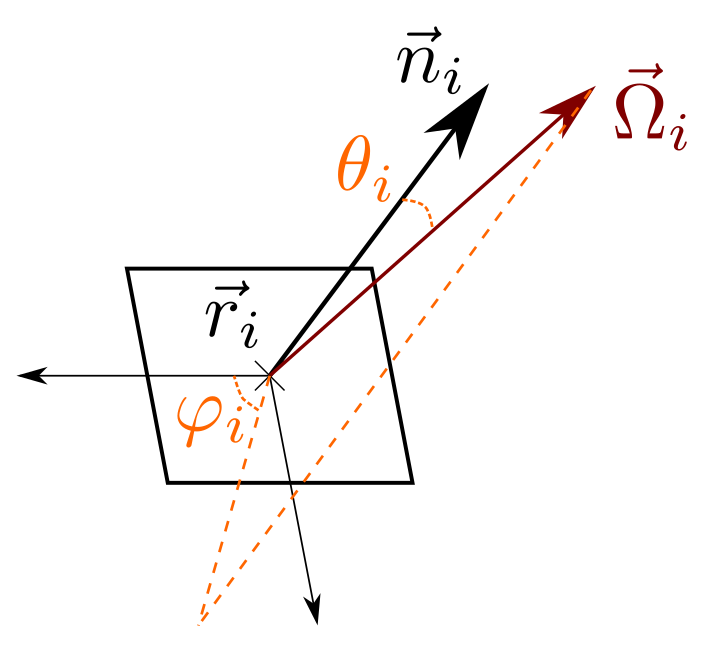
\includegraphics[width = 0.3\linewidth]{PICTURES/HS_schema.png}
    \caption{Illustration des notations géométriques introduites à l'Eq \ref{def:fv_mcrt}}
    \label{fig:fij_schema}
\end{figure}

La première étape est de faire un tirage naïf de la position et de la direction du rayon. Les stratégies d'échantillonage et de stratification seront dévelopées dans la Partie \ref{part:echanti}. L'estimateur naïf est donc construit comme suit :
\begin{equation}
    \hat{F_{ij}}^N =   \frac{1}{N} \sum_{n = 1}^{N} \hat{F}_{ij}^{n} \quad \text{avec } \hat{F}_{ij}^{n} = 1_{A_j}(\vec{r_i}^{n}, \vec{\Omega_i}^{n}) 
\label{def:fv_mc}
\end{equation}

Une variance non biaisé de l'estimateur se construit de la même manière : 
\begin{equation}
    \hat{V_{ij}}^N =   \frac{1}{N-1} \Big( \frac{1}{N} \sum_{n = 1}^{N}   [ \hat{F}_{ij}^{n} - \hat{F}_{ij}^N]^2    \Big)
\end{equation}
